
%% this section contains XX problems


%% 2004-APB
%%------------------------------
\element{AP}{
\begin{question}{2004-APB-Q26}
    An object is placed in front of a converging thin lens at a distance
        from the center of the lens equal to half the focal length.
    Compared to the object, the image is
    \begin{choices}
      \correctchoice{upright and larger}
        \wrongchoice{upright and smaller}
        \wrongchoice{inverted and larger}
        \wrongchoice{inverted and smaller}
        \wrongchoice{inverted and the same size}
    \end{choices}
\end{question}
}

\element{AP}{
\begin{question}{2004-APB-Q27}
    A radio station broadcast on a carrier frequency
        of \SI{100}{\mega\hertz}.
    The wavelength of this radio wave is most nearly
    \begin{multicols}{3}
    \begin{choices}
        \wrongchoice{\SI{3.0e-3}{\meter}}
        \wrongchoice{\SI{1.0}{\meter}}
      \correctchoice{\SI{3.0}{\meter}}
        \wrongchoice{\SI{3.3}{\meter}}
        \wrongchoice{\SI{3.0e6}{\meter}}
    \end{choices}
    \end{multicols}
\end{question}
}

\element{AP}{
\begin{question}{2004-APB-Q50}
    A light ray $R$ in medium I strikes a sphere of medium II
        with angle of incidence $\theta$, as shown below.
    The figure shows five possible subsequent paths for the light ray.
    \begin{center}
        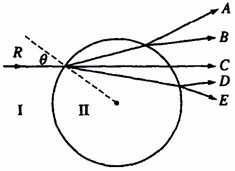
\includegraphics[keepaspectratio]{2004-APB-Q50}
    \end{center}
    Which path is possible if medium I is air and medium II is glass?
    \begin{multicols}{3}
    \begin{choices}
        \wrongchoice{$A$}
        \wrongchoice{$B$}
        \wrongchoice{$C$}
      \correctchoice{$D$}
        \wrongchoice{$E$}
    \end{choices}
    \end{multicols}
\end{question}
}

\element{AP}{
\begin{question}{2004-APB-Q51}
    A light ray $R$ in medium I strikes a sphere of medium II
        with angle of incidence $\theta$, as shown below.
    The figure shows five possible subsequent paths for the light ray.
    \begin{center}
        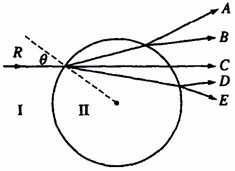
\includegraphics[keepaspectratio]{2004-APB-Q50}
    \end{center}
    Which path is possible if medium I is glass and medium II is air?
    \begin{multicols}{3}
    \begin{choices}
        \wrongchoice{$A$}
      \correctchoice{$B$}
        \wrongchoice{$C$}
        \wrongchoice{$D$}
        \wrongchoice{$E$}
    \end{choices}
    \end{multicols}
\end{question}
}

\element{AP}{
\begin{question}{2004-APB-Q53}
    A thin film with index of refraction $n_f$ separates two materials,
        each of which has an index of refraction less than $n_f$.
    A monochromatic beam of light is incident normally on the film,
        as shown above.
    If the light has wavelength $\lambda$ within the film, maximum
        constructive interference between the incident beam and the
        reflected beam occurs for which of the following film thicknesses?
    \begin{multicols}{3}
    \begin{choices}
        \wrongchoice{$3 \lambda$}
        \wrongchoice{$2 \lambda$}
        \wrongchoice{$\lambda$}
      \correctchoice{$\dfrac{\lambda}{2}$}
        \wrongchoice{$\dfrac{\lambda}{4}$}
    \end{choices}
    \end{multicols}
\end{question}
}

\element{AP}{
\begin{question}{2004-APB-Q54}
    An object is placed on the axis of a converging thin lens of focal
        length \SI{2}{\centi\meter}, at a distance of \SI{8}{\centi\meter}
        from the lens.
    The distance between the image and the lens is most nearly
    \begin{multicols}{3}
    \begin{choices}
        \wrongchoice{\SI{0.4}{\centi\meter}}
        \wrongchoice{\SI{0.8}{\centi\meter}}
        \wrongchoice{\SI{1.6}{\centi\meter}}
        \wrongchoice{\SI{2.0}{\centi\meter}}
      \correctchoice{\SI{2.7}{\centi\meter}}
    \end{choices}
    \end{multicols}
\end{question}
}

\element{AP}{
\begin{question}{2004-APB-Q55}
    A large lens is used to focus an image of an object onto a screen.
    If the left half of the lens is covered with a dark card, which of
        the following occurs?
    \begin{choices}
        \wrongchoice{The left half of the image disappears.}
        \wrongchoice{The right half of the image disappears.}
        \wrongchoice{The image becomes blurred.}
      \correctchoice{The image becomes dimmer.}
        \wrongchoice{No image is formed}
    \end{choices}
\end{question}
}

\element{AP}{
\begin{question}{2004-APB-Q60}
    A \SI{50 000}{\watt} radio station transmits waves
        of wavelength \SI{4}{\meter}.
    Which of the following is the best estimate of the number
        of photons it emits per second?
    \begin{multicols}{3}
    \begin{choices}
        \wrongchoice{\num{e8}}
        \wrongchoice{\num{e22}}
      \correctchoice{\num{e30}}
        \wrongchoice{\num{e40}}
        \wrongchoice{\num{e56}}
    \end{choices}
    \end{multicols}
\end{question}
}


